\chapter{Desenvolvimento da Solução}
\label{chap:solucaocompleta}

\section{Metodologia}

Esse trabalho está dentro de um contexto específico na engenharia de software. Esse contexto se caracteriza num projeto de pesquisa e desenvolvimento no qual até a consolidação da solução pouco se sabia sobre sua natureza (por exemplo arquitetura e viabilidade), o andamento do desenvolvimento ocorreu de forma não-linear e complexa e houve um frequente diálogo entre disciplinas de diferentes domínios - transdiciplinaridade.

No que diz respeito ao desconhecimento da natureza da solução no início do projeto, houve várias questões teóricas de pesquisa que foram passíveis de experimentações e disscusões ao longo do processo de desenvolvimento. Tal fato ocasionou na caracterização da solução ao longo do projeto e sua definição total somente no final.

No que tange a não-linearidade, variou-se muito o desempenho na concretização de soluções. A taxa de produção intelectual comportou-se como não repetível ao longo do tempo. E a complexidade, de acordo com a teoria de Edgar Morin \cite{morin}, impactou o projeto de forma que a soma dos métodos e tecnologias gerasse resultados imprevisíveis.

O termo transdisciplinaridade é empregado para um patamar de relações entre disciplinas e domínios de conhecimento. Conceitua-se como tal um processo que transcende as disciplinas, que está entre, além e através das disciplinas \cite{criatividade}. Nesse trabalho foram investigados vários domínios de conhecimento como a engenharia, matemática, neurociências, psicologia, música e computação.

Dado o contexto e características do trabalho foi estabelicido um método de desenvolvimento empírico, iterativo e incremental.

Na engenharia de software se destacam dois processos de controle de desenvolvimento: precesso definido e processo empírico. O processo definido é constiuído de um conjunto de sub-processos rigoros nos quais possuem entradas e saídas bem definidas e repetitivas \cite{rup}. Já o processo empírico é constituído de um conjunto de sub-processos imperfeitamente definidos nos quais as entradas e saídas são imprevisíveis e não repetíveis, características essas presentes no desenvolvimento desse trabalho.

A metodologia empírica de desenvolvimento de software se embasa três fundamentos: precisa ser transparente, visto que o máximo de variáveis devem estar visíveis para os envolvidos no projeto; dado as variáveis expostas a metodologia precisa ser frequentemente inspecionada; feito as inspeções objetivo final é adaptar de acordo com as necessidades. Esses três fundamentos visam ajustar o processo de desenvolvimento para evitar variações de produção inaceitáveis e maximizar a mesma \cite{empirical}.

Para que os procedimentos da metodologia empírica possa ocorrer ela precisa ser de natureza iterativa e incremental. Iterativa e incremental pois terá ciclos curtos de desenvolvimento e a cada ciclo terá incrementos de código. No final de cada ciclo ter-se-à como resultado parâmetros de feedback para a melhoria contínua.

Outra análise do método empírico é o embasamento no ciclo de melhoria de processos e produtos $Plan$-$Do$-$Check$-$Act$ (PDCA) \cite{pdca}. Ele é constuído em 4 fases: $Plan$ - planejamento do desenvolvimento; $Do$ - executar o que foi planejado; $Check$ - avaliar o que foi feito; $Act$ - propor melhorias para os próximos ciclos.

Por fim, para consolidação da metodologia abordada nesse trabalho, foi utilizado o modelo $Goal$-$Question$-$Metric$ (GQM) para a estruturação dos ciclos \cite{gqm}. Esse modelo foi utilizado para orientar o desenvolvimento e ele é composto por 3 etapas sucessivas: $Goal$ - objetivo a ser alcançado; $Question$ - questões chaves para que o objetivo possa ser alcançado; $Metric$ - métricas que vão validar se as questões foram respondidas e objetivo alcançado. Nesse contexto os objetivos do trabalho são os objetivos específicos, as questões são as hipotéses levantadas no início de cada ciclo e as métricas são os resultados finais de cada ciclo.

% QUESTÕES
Com o intuito de atingir os objetivos, serão abordados questões, hipóteses e critérios relacionados às problemáticas abordadas. No que diz respeito as questões, segue a formulação das mesmas:
\begin{itemize}
	\item Se cada nota é uma frequência de vibração sonora, como analisar o sinal no ponto de vista de frequências? Dessa questão, surge a seguinte hipótese:
	\begin{itemize}
		\item A transformada de fourier pode construir o espectro de frequências do sinal. O critério para avaliar essa hipótese é:
			\begin{itemize}
				\item Vetor com os níveis de energia relacionados a cada frequência.		
			\end{itemize}
	\end{itemize}

	\item Como configurar essas informações para localizar as notas musicais?
	\begin{itemize}
		\item Dado que cada nota musical é um conjunto de frequências, realocar as energias frequenciais da transformada de fourier afim de que cada posição do vetor seje 1 unidedade de frequência (Hz) pode mapear a energia de cada nota. Os critérios para avaliar essa hipótese são:
			\begin{itemize}
				\item Vetor com os níveis de energia relacionados a cada frequência deve ter o tamanho de 22050 posições.
				\item Cada posição do vetor de energia relacionados a cada frequência possui valor de 1 Hz.		
			\end{itemize}
	\end{itemize}

	\item Como adicionar as próximas camadas da rede para determinação dos acordes?
	\begin{itemize}
		\item  Visto que associar as frequências as notas musicas é uma tarefa muito complexa para uma solução determinística, uma rede neural de aprendizado não supervisionado do tipo $Probabilistic Neural Network$ (PNN) pode classificar um conjunto de frequências em sua respectiva nota musical. O critério para avaliar essa hipótese é:
			\begin{itemize}
				\item Vetor com os níveis de energia relacionados a cada nota.		
			\end{itemize}
	\end{itemize}
	
	\item Como reconhecer acordes no tempo de tal forma a saber onde eles ocorrem?
	\begin{itemize}
		\item A transformada de fourier pode construir o espectro de frequências do sinal.
		O critério para avaliar essa hipótese é:
			\begin{itemize}
				\item Vetor com os níveis de energia relacionados a cada frequência.		
			\end{itemize}
	\end{itemize}
	\item Como ler o sinal todo e ter a visilibilidade em tempo e frequência?
	\begin{itemize}
		\item A transformada de fourier pode construir o espectro de frequências do sinal.
		O critério para avaliar essa hipótese é:
			\begin{itemize}
				\item Vetor com os níveis de energia relacionados a cada frequência.		
			\end{itemize}
	\end{itemize}
	\item Como ler o sinal todo e ter a visilibilidade em tempo e frequência?
	\begin{itemize}
		\item A transformada de fourier pode construir o espectro de frequências do sinal.
		O critério para avaliar essa hipótese é:
			\begin{itemize}
				\item Vetor com os níveis de energia relacionados a cada frequência.		
			\end{itemize}
	\end{itemize}
	\item Como extrair o tom da música?
	\begin{itemize}
		\item A transformada de fourier pode construir o espectro de frequências do sinal.
		O critério para avaliar essa hipótese é:
			\begin{itemize}
				\item Vetor com os níveis de energia relacionados a cada frequência.		
			\end{itemize}
	\end{itemize}
	\item Como trabalhar com a frequência de aparecimento das notas?
	\begin{itemize}
		\item A transformada de fourier pode construir o espectro de frequências do sinal.
		O critério para avaliar essa hipótese é:
			\begin{itemize}
				\item Vetor com os níveis de energia relacionados a cada frequência.		
			\end{itemize}
	\end{itemize}
	\item Em relação aos acordes transitórios, como corrigir?
	\begin{itemize}
		\item A transformada de fourier pode construir o espectro de frequências do sinal.
		O critério para avaliar essa hipótese é:
			\begin{itemize}
				\item Vetor com os níveis de energia relacionados a cada frequência.		
			\end{itemize}
	\end{itemize}
	\item Como extrair a nota mais grave (baixo) de cada período do tempo?
	\begin{itemize}
		\item A transformada de fourier pode construir o espectro de frequências do sinal.
		O critério para avaliar essa hipótese é:
			\begin{itemize}
				\item Vetor com os níveis de energia relacionados a cada frequência.		
			\end{itemize}
	\end{itemize}
	\item Como extrair a nota mais grave (baixo) de cada período do tempo e incluir os acordes aumentados e invertidos?
	\begin{itemize}
		\item A transformada de fourier pode construir o espectro de frequências do sinal.
		O critério para avaliar essa hipótese é:
			\begin{itemize}
				\item Vetor com os níveis de energia relacionados a cada frequência.		
			\end{itemize}
	\end{itemize}
\end{itemize}


\section{Técnicas Utilizadas para Desenvolvimento do Sistema-Solução}

Nesta secção será descrito o desenvolvimento da solução e as técnicas utilizadas. A explicação da solução se embasará no seguinte diagrama de fluxo de dados:

\begin{figure}[h]
	\centering
		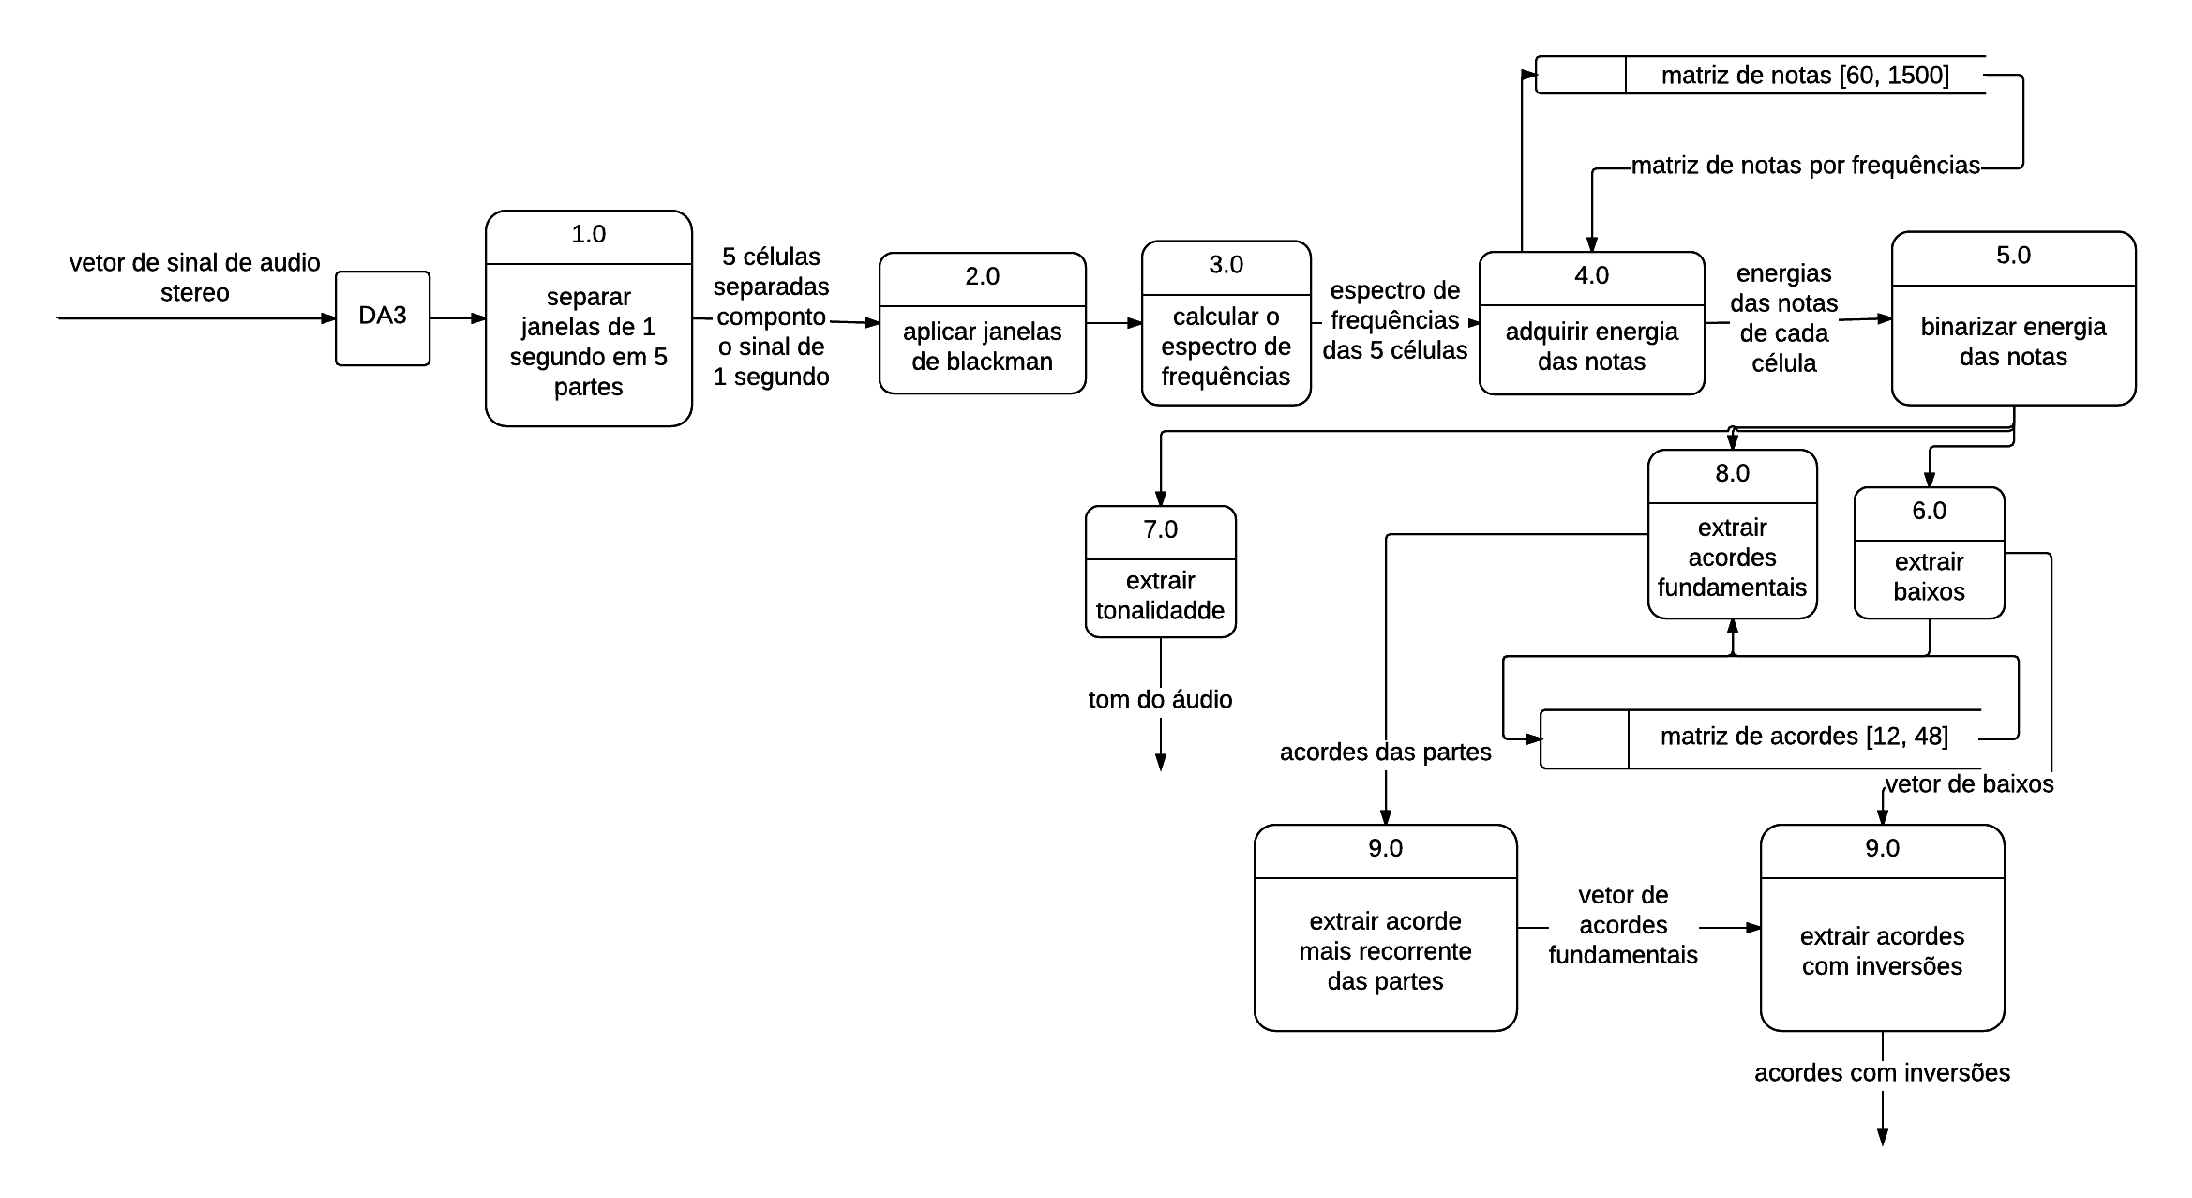
\includegraphics[keepaspectratio=true,scale=0.51]{figuras/dfd_2.eps}
	\caption{Diagrama de Fluxo de Dados}
\end{figure}

A solução começa com a chamada da função DA3. Ela recebe como parâmetro um vetor de audio $stereo$, ou seja, ela carrega uma matriz 2 por N, tal que N é o tamanho do sinal de áudio (número de amostras). Esse sinal de áudio é retornado através da função $wavread$($<$$caminho$ $do$ $arquivo$$>$$)$. O tipo de arquivo lido é do formato-padrão de áudio .wav. Esse formato de arquivo permite um armazenamento dos dados em blocos em modulação de pulsos PCM ($pulse$-$code$-$modulation$). O PCM armazena em arquivo de áudio não-comprimido (sem perdas), ou seja, o processo de amostragem e quantização representa exatamente o que foi descrito na parte de fundamentos teóricos desse trabalho (taxa de amostragem de 44.100 Hz e quantização de 16 bits). Ao final do fluxo há 2 saídas: os acordes ao longo do tempo e o tom do áudio.Nos próximos tópicos serão explicados os comportanmentos de cada uma das caixas de processamento do diagrama de fluxo de dados.

\subsection{Procedimento 1: Separar Janelas de 1 Segundo em 5 Partes}
\label{sec:janelas}

Após o sinal ser carregado num vetor de audio $stereo$, ele deverá ser transformado num do tipo mono. Sinal mono de áudio é aquele com somente um canal. Isso é necessário para que o processamento não fosse redundante. Não agregaria valor nesse caso processar um sinal de duplo canal sendo que a fonte emissora de ondas sonoras é comum para ambos. Após essa conversão o sinal é repartidos em 5 partes de tamanhos iguais a 1 segundo, porém deslocadas a 0.2 segundos de cada um. Esse processo é para a segmentar áudio no intuito de achar o acorde mais provável num intervalo de tempo de um segundo, fazendo com que acordes de transição ou ruidosos sejam suprimidos. Esse procedimento pode ser conferido a seguir:
\begin{lstlisting}
% get total seconds of time to mensure the length of music 
signal = signal(:,1);
time_seconds_total = fix((length(signal)/fs)); 

% preparing struct to allocate notes in time
set_of_notes_time = {};
for set = 1:5
    notes_time(time_seconds_total, 60) = 0;
    set_of_notes_time{set} = notes_time;
end
\end{lstlisting}

Basicamente a variável de entrada dessa função é reescrita como uma matriz 1 por N, tal qual N é o número de amostras do sinal. No laço seguinte cria-se um conjunto de 5 células, cada uma comportando uma parte do sinal.

\subsection{Procedimento 2: Aplicar Janelas de Blackman}
\label{sec:transformada}

Dado que o contexto da solução se deu por $Short$-$Time$-$Fourier$-$Transform$, é preciso minimizar as distorções oriundas dos janelamentos. Para tal foi proposto a multiplicação de cada parte das janelas ao longo do tempo por uma janela de blackman, uma do tipo gaussiana. Segue procedimento em código abaixo:
\begin{lstlisting}
function set_of_windows_signals = build_window_short_fft(signal, time, fs)
	signal = [signal(:)];

    % part A
    time_start_A = round(1+((time-1)*fs));
    time_end_A = round(time*fs);
    signal_time_A = signal(time_start_A:time_end_A);
    signal_time_A = blackman(length(signal_time_A)).*signal_time_A;

    % part B (displacement = + 0.2 seconds)
    time_start_B = round(1+((time-1)*fs+0.2*fs));
    time_end_B = round((time+0.2)*fs);
    if time_start_B < length(signal) && time_end_B <= length(signal)
        signal_time_B = signal(time_start_B:time_end_B);
        signal_time_B = blackman(length(signal_time_B)).*signal_time_B;
    else
        signal_time_B(length(signal)) = 0;
    end

    % part C (displacement = + 0.4 seconds)
    time_start_C = round(1+((time-1)*fs+0.4*fs));
    time_end_C = round((time+0.4)*fs);
    if time_start_C < length(signal) && time_end_C <= length(signal)
        signal_time_C = signal(time_start_C:time_end_C);
        signal_time_C = blackman(length(signal_time_C)).*signal_time_C;
    else
        signal_time_C(length(signal)) = 0;
    end

    % part D (displacement = + 0.6 seconds)
    time_start_D = round(1+((time-1)*fs+0.6*fs));
    time_end_D = round((time+0.6)*fs);
    if time_start_D < length(signal) && time_end_D <= length(signal)
        signal_time_D = signal(time_start_D:time_end_D);
        signal_time_D = blackman(length(signal_time_D)).*signal_time_D;
    else
        signal_time_D(length(signal)) = 0;
    end

    % part E (displacement = + 0.8 seconds)
    time_start_E = round(1+((time-1)*fs+0.8*fs));
    time_end_E = round((time+0.8)*fs);
    if time_start_E < length(signal) && time_end_E <= length(signal)
        signal_time_E = signal(time_start_E:time_end_E);
        signal_time_E = blackman(length(signal_time_E)).*signal_time_E;
    else
        signal_time_E(length(signal)) = 0;
    end

    set_of_windows_signals = {};
    if length(signal_time_A) == length(signal_time_B) && ...
        length(signal_time_A) == length(signal_time_C) && ...
         length(signal_time_A) == length(signal_time_D) &&  ...
          length(signal_time_A) == length(signal_time_E)
        set_of_windows_signals{1} = signal_time_A;
        set_of_windows_signals{2} = signal_time_B;
        set_of_windows_signals{3} = signal_time_C;
        set_of_windows_signals{4} = signal_time_D;
        set_of_windows_signals{5} = signal_time_E;
    else
        set_of_windows_signals{1} = signal_time_A;
        set_of_windows_signals{2} = signal_time_A;
        set_of_windows_signals{3} = signal_time_A;
        set_of_windows_signals{4} = signal_time_A;
        set_of_windows_signals{5} = signal_time_A;
    end
\end{lstlisting}

\subsection{Procedimento 3: Calcular o Espectro de Frequências}

O passo seguinte é adquirir os espectros de frequências oriundos do cálculo da transformada discreta de fourier. O cálculo será feito para cada uma das 5 partes de janelas. Segue procedimentos para tal:
\begin{lstlisting}
	% get frequency spectrum
function set_of_spectrums = get_frequency_spectrum( ...
set_of_windows_signals, sampling)

    % allocate struct to spectrum
    set_of_spectrums = {};
    sampling = sampling/21;

    for part_signal_iterator = 1:5
    	% make downsample to put frequency max in 1050 Hz
        signal = downsample(set_of_windows_signals{ ...
part_signal_iterator}, 21);
        % doing fourier transform
        frequencies=(0:length(signal)-1)*sampling/length(signal);
        module_fft = abs(fft(signal));
        f_round = round(frequencies);
        frequencies_energy(max(f_round)) = 0;
        for slot = 2:length(f_round)
            frequencies_energy(f_round(slot)) = module_fft(slot);
        end
        frequency_spectrum_part = frequencies_energy(1:fix(end/2));
        set_of_spectrums{part_signal_iterator} = frequency_spectrum_part;
    end
\end{lstlisting}

Primeiramente é alocado uma variável para comportar os 5 espectros de frequência, um para cada parte da janela. Depois os sinais passam por uma transformação de subamostragem na qual são eliminadas informações de altas frequências a partir de 1500 Hz. É feito o cálculo do módulo da transformada de frourier e esse mesmo vetor passar por uma reorganização de $slots$ de tal forma que cada $slot$ comporta-se 1 unidade de Hz.

\subsection{Procedimento 4: Adquirir Energias das Notas}

Nesse procedimento cada espectro de frequência é correlacionado com conjunto de notas musicais dado um conjunto de frequências que nelas estão presentes. Ao final do processo espera-se matrizes de conjuntos de notas para cada uma das 5 partes da janela. Segue os procedimentos em código feitos:
\begin{lstlisting}
function set_of_notes_time = get_energy_notes(set_of_spectrums, ...
set_of_notes_time, time)
	
	% load data notes
	load_notes;

	for set = 1:5
		respfreq = set_of_spectrums{set};
		notes_time = set_of_notes_time{set};

		% this case works in one case
		respfreq = [respfreq zeros(1, length(notes(1,:)) - ...
length(respfreq))];
		for note = 1:60
	        notes_time(time, note) = sum((respfreq.*notes(note,:)).^2);    
		end	

		set_of_notes_time{set} = notes_time;
	end
\end{lstlisting}

A primeira atividade é carregar a base de dados de notas musicais originando o retorno de um matriz 60 notas por 1500 frequências. Então cada conjunto de notas relacionados às partes de janela serão correlacionados a partir de uma operação de multiplicação e, por fim, é feita a soma dos quadrados dos termos. Ao final uma matriz de notas por tempo é construída para cada uma das 5 partes.

\section{Procedimento 5: Binarizar Energia das Notas}

Esse passo compreende o processo de limiarização das energias das notas em 0's ou 1's de tal forma que se possa detectas as notas tocadas (1) ou não (0). Ao final desse processo espera-se conjuntos de energias de notas musicais em somente dois valores - 1 ou 0. Segue o código para esse processo:
\begin{lstlisting}
% binarize set of notes
    for set = 1:5
        notes_time = set_of_notes_time{set};
        
        for time = 1:time_seconds_total
            for note = 1:60
                if notes_time(time, note) < max(max(notes_time))/180
                    notes_time(time, note) = 0;
                else
                    notes_time(time, note) = 1;
                end
            end
        end

        set_of_notes_time{set} = notes_time;
    end
\end{lstlisting}

No começo do procedimento é destacado um laço para cada uma das partes das janelas. No meio do procedimento destaca-se com operação de realocação do valor 0 para valores de energia menores que 180\% do valor máximo do conjunto de notas e 1 se for caso ao contrário. Por fim cada conjunto de notas são realocados em células.

\section{Procedimento 6: Extrair Baixos}

Com o intuito de determinar acordes com inversões e discernir os que são de natureza aumentada, acoplou-se no sistema um componente desenvolvido para a extração das notas mais graves numa dada janela de tempo. Segue o código desenvolvido para essa atividade:
\begin{lstlisting}
function bass_time = get_bass(set_of_notes_time)

	notes_time_A = set_of_notes_time{1};
	notes_time_B = set_of_notes_time{2};
	notes_time_C = set_of_notes_time{3};
	notes_time_D = set_of_notes_time{4};
	notes_time_E = set_of_notes_time{5};

	total_seconds = length(notes_time_A(:,1));
	notes_time(total_seconds, 60) = 0;
	for time = 1:total_seconds
		for note = 1:60
			notes_to_analyse = [notes_time_A(time, note) ...
			 notes_time_B(time, note) ...
		 notes_time_C(time, note) ...
		  notes_time_D(time, note) ...
		   notes_time_E(time, note)];
			notes_time(time, note) = mode(notes_to_analyse);
		end
	end

    bass_time(1:total_seconds) = 0;
	for time = 1:total_seconds
		maxs = find(notes_time(time,:)==max(notes_time(time,:)));
		bass_time(time) = maxs(1);
	end

	for bass = 1:length(bass_time)
		bass_time(bass) = mod(bass_time(bass) - 1, 12) + 1;
	end

end
\end{lstlisting}

No procedimento verificamos que os primeiros passos são de atribuição de variáveis em relação as partes das janelas. Depois cada uma dessas partes serão analisadas quanto as notas mais recorrentes com a função \textbf{mode}. Dado essa análise os baixos são extraidos com a primeira ocorrência de 1, dado que as notas estão binarizadas.

\subsection{Procedimento 7: Extrair Tonalidade}

A extração de tonalidade é um módulo do sistema que possui como entrada o conjunto de notas binarizadas das partes de janela. A saída é o tom da música tocado baseando-se em acordes fundamentais maiores e menores. Segue a especificação do procedimento:
\begin{lstlisting}
function [chord_pitch, chord_pitch_number] = ...
get_chord_pitch(notes_time, time_seconds_total, chords)
	
	dictionary_chords = { 'C', 'Cm', 'Caum', 'Cdim', ...
     'C#', 'C#m', 'C#aum', 'C#dim', 'D', 'Dm', 'Daum', 'Ddim', ...
     'Eb', 'Ebm', 'Ebaum', 'Ebdim', 'E', 'Em', 'Eaum', 'Edim', ...
     'F', 'Fm', 'Faum', 'Fdim', 'F#', 'F#m', 'F#aum', 'F#dim', ...
     'G', 'Gm', 'Gaum', 'Gdim', 'G#', 'G#m', 'G#aum', 'G#dim', ...
     'A', 'Am', 'Aaum', 'Adim', 'Bb', 'Bbm', 'Bbaum', 'Bbdim', ...
     'B', 'Bm', 'Baum', 'Bdim' };

	notes_energy_total(60) = 0;
	for note = 1:60
		notes_energy_total(note) = sum([notes_time(:,note)]);
	end

	% discover tone music
	notes_energy_tone(12) = 0;
	for note = 1:12
		notes_energy_tone(note) = notes_energy_total(note) + ...
		 notes_energy_total(note + 12) ...
			+ notes_energy_total(note + 2*12) + ...
			 notes_energy_total(note + 3*12) ...
				+ notes_energy_total(note + 4*12);
	end

	% find chord tone
	load_chords_tone;
	chords_tone(48) = 0;
	for chord = 1:48
		chords_tone(chord) = sum((notes_energy_tone.* ...
			 chords_tone_mask(:, chord)'.^2));
	end

	chord_pitch_number = find(chords_tone==max(chords_tone));
	chord_pitch = dictionary_chords{chord_pitch_number};

\end{lstlisting}

No início desse processo há declaração nominal dos acordes em tipo string. Após o conjunto de notas em relação são somadas, cada uma na sua respectiva frequência, para gerar um vetor que totaliza a soma das frequências tocadas ao longo de todo áudio. O procedimento seguinte, focando extrair um acorde desse vetor de notas ao longo de todo áudio, é utilizado uma correlação do mesmo com uma base dados carregada de notas pelos respectivos acordes. Ao final cada acorde da base de dados terá sua energia correspondente e, ao extrair o máximo das energias, é adquirido o acorde tom da música.

\section{Procedimento 8: Extrair Acordes Fundamentais}

A extração de acordes fundamentais é um módulo do sistema que possui como entrada o conjunto de notas binarizadas das partes de janela. A saída é um conjunto de acordes fundamentais ao longo do tempo. Segue a especificação do procedimento:
\begin{lstlisting}
function set_of_chords_time = get_set_of_chords_time(set_of_notes_time)
	load_chords_tone;

	set_of_chords_time = {};
	for set = 1:5
		notes_time = set_of_notes_time{set};
		time_total = length(notes_time(:,1));
		chords_time(1:time_total) = 0;

		for time = 1:time_total
			
			notes_energy_tone(12) = 0;
			for note = 1:12
				notes_energy_tone(note) = notes_time(time, note) + ... 
				notes_time(time, note + 12) ...
					+ notes_time(time, note + 2*12) + ...
					 notes_time(time, note + 3*12) ...
						+ notes_time(time, note + 4*12);
			end

			energy_chords(1:48) = 0;
		    for chord = 1:48
		        energy_chords(chord) = sum((notes_energy_tone.* ...
		        		chords_tone_mask(:, chord)').^2);
		    end
		    
		    max_chord = find(energy_chords==max(energy_chords));

		    chords_time(time) = max_chord(1);
		end

		set_of_chords_time{set} = chords_time;
	end
end
\end{lstlisting}

No início desse processo há o carregamento da base de dados de acordes em relação as notas musicais. Após o conjunto de notas são somadas em relação às respectivas oitavas gerando vetor de somente 12 posições. Esse mesmo vetor é submetido então a um processo de correlação aos acordes derivados da base de dados. Ao final cada acorde da base de dados terá sua energia correspondente e, ao extrair o máximo das energias, é adquirido os acordes fundamentais ao longo do tempo.

\section{Procedimento }

Depois desse processo há 2 vetores que compõem a representação do módulo espectral, ambos com tamanho igual a metade da quantidade de amostras do sinal original: vetor de frequências e vetor do módulo da transformada de fourier. É desejável para o andamento do processo um vetor de módulo frequencial com o tamanho de 22.050 posições. Esse tamanho é necessário para representar a energia da função de base (senóide) somente acessando a posição do vetor, por exemplo: para saber qual a energia da onda senoidal de 440 Hz é só acessar a posição 440 desse mesmo vetor. Para tal construiu-se o seguinte código:
\begin{lstlisting}
	i = 1;
	j = 0;
	l = 1;
	SOMA = 0;
	while (i<length(freq))
    	if (round(freq(i)) == round(freq(i+1)))
        	SOMA = SOM(i+1) + SOMA;
        	j = j + 1;
   	 	else
        	respfreq(l) = SOMA/(j+1);
        	j = 0;
        	SOMA = SOM(i+1);
        	l = l+1;
    	end
    	i = i+1;
	end
\end{lstlisting}

A variável \textbf{i} representa um iterador para todas as posições do vetor das frequências. A variável \textbf{j} representa uma faixa de frequências, que arredondando as mesmas, são equivalentes. A variável \textbf{l} representa a quantidade total de faixas de frequências, que arredondando as mesmas, são equivalentes de tal forma que \textbf{l}x\textbf{j} = \textbf{i}. A variável \textbf{SOMA} possui a responsabilidade de popular a energia dessas frequências congruentes em cada posição do novo vetor. Esse laço de repetição vai passar pela totalidade das frequências e em cada posição verificará as frequências equivalentes via arredondamento. A medida que se vai encontrando determinadas frequências congruentes, uma posição do valor de energia da transformada de fourier é somada. Quando a próxima frequência não é mais congruente com a anterior, o vetor \textbf{respfreq} recebe a média ponderada dessas energias.

O resultado desse processamento é ilustrado a seguir:

\begin{figure}[h]
	\centering
		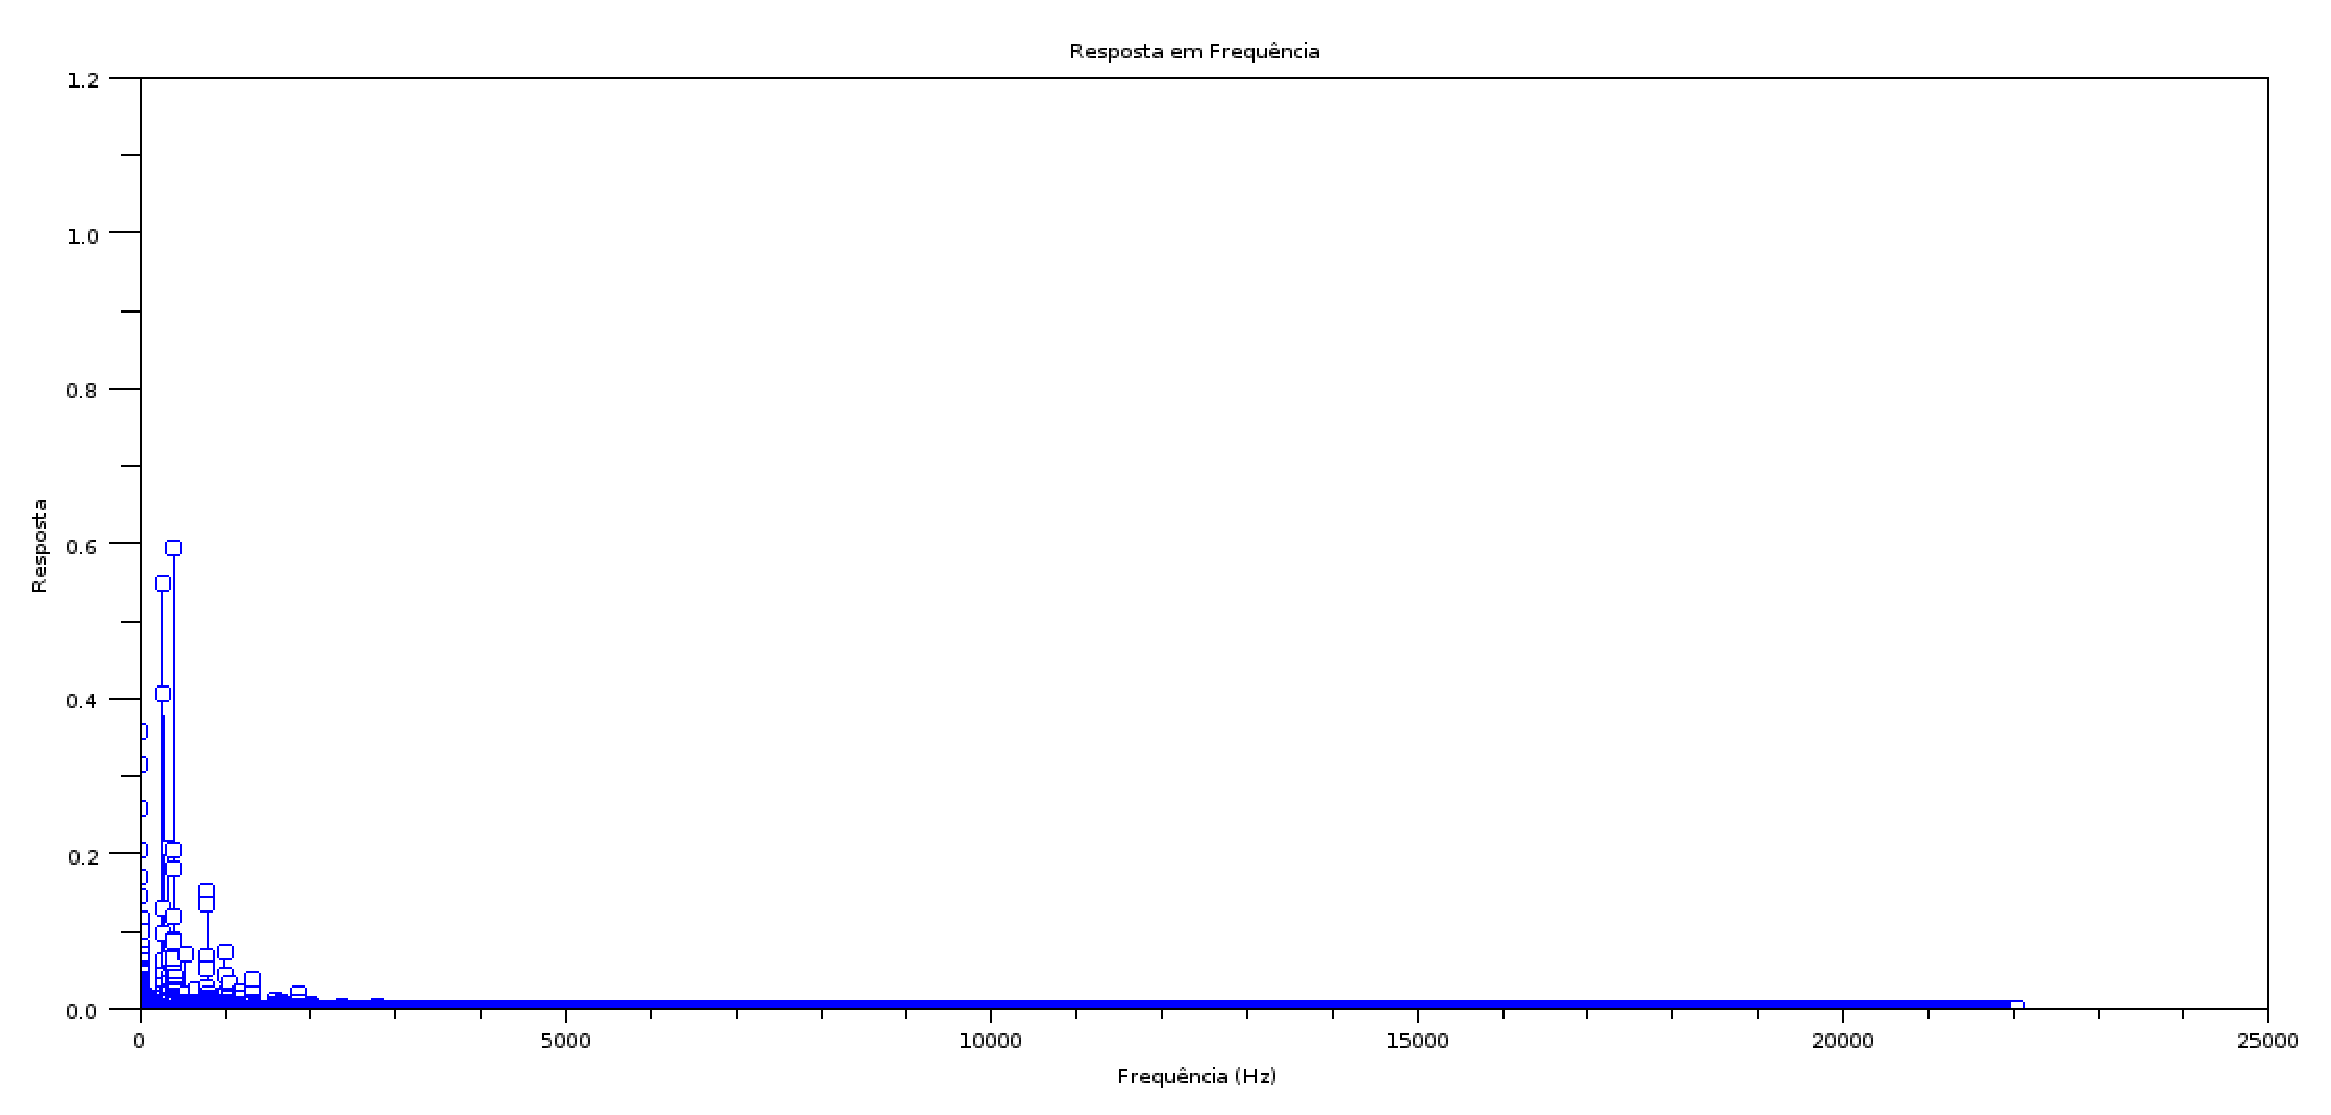
\includegraphics[keepaspectratio=true,scale=0.45]{figuras/fft-resultado}
	\caption{Vetor de 22.050 posições de Resposta em Frequência}
\end{figure}

O espectro de frequências está mais concentrado no lado esquerdo de todos os valores de frequências possíveis e audíveis ao ouvido humano. Esse fato é explicado devido ao uso de notas musicais serem usadas normalmente de 60 Hz a 3000 Hz.

\newpage
\section{Correlação com Notas Musicais}
\label{sec:correlacaonotas}

Na função de correlacionar o espectro de frequência com as notas musicais há a presença de uma estrutura de uma rede neural. Para essa rede foram criados 12 neurônios, 1 para cada nota musical. Segue um exemplo de esquema de um neurônio para a nota $Dó$, para as outras notas segue a mesma estrutura de neurônio:

\begin{figure}[h]
	\centering
		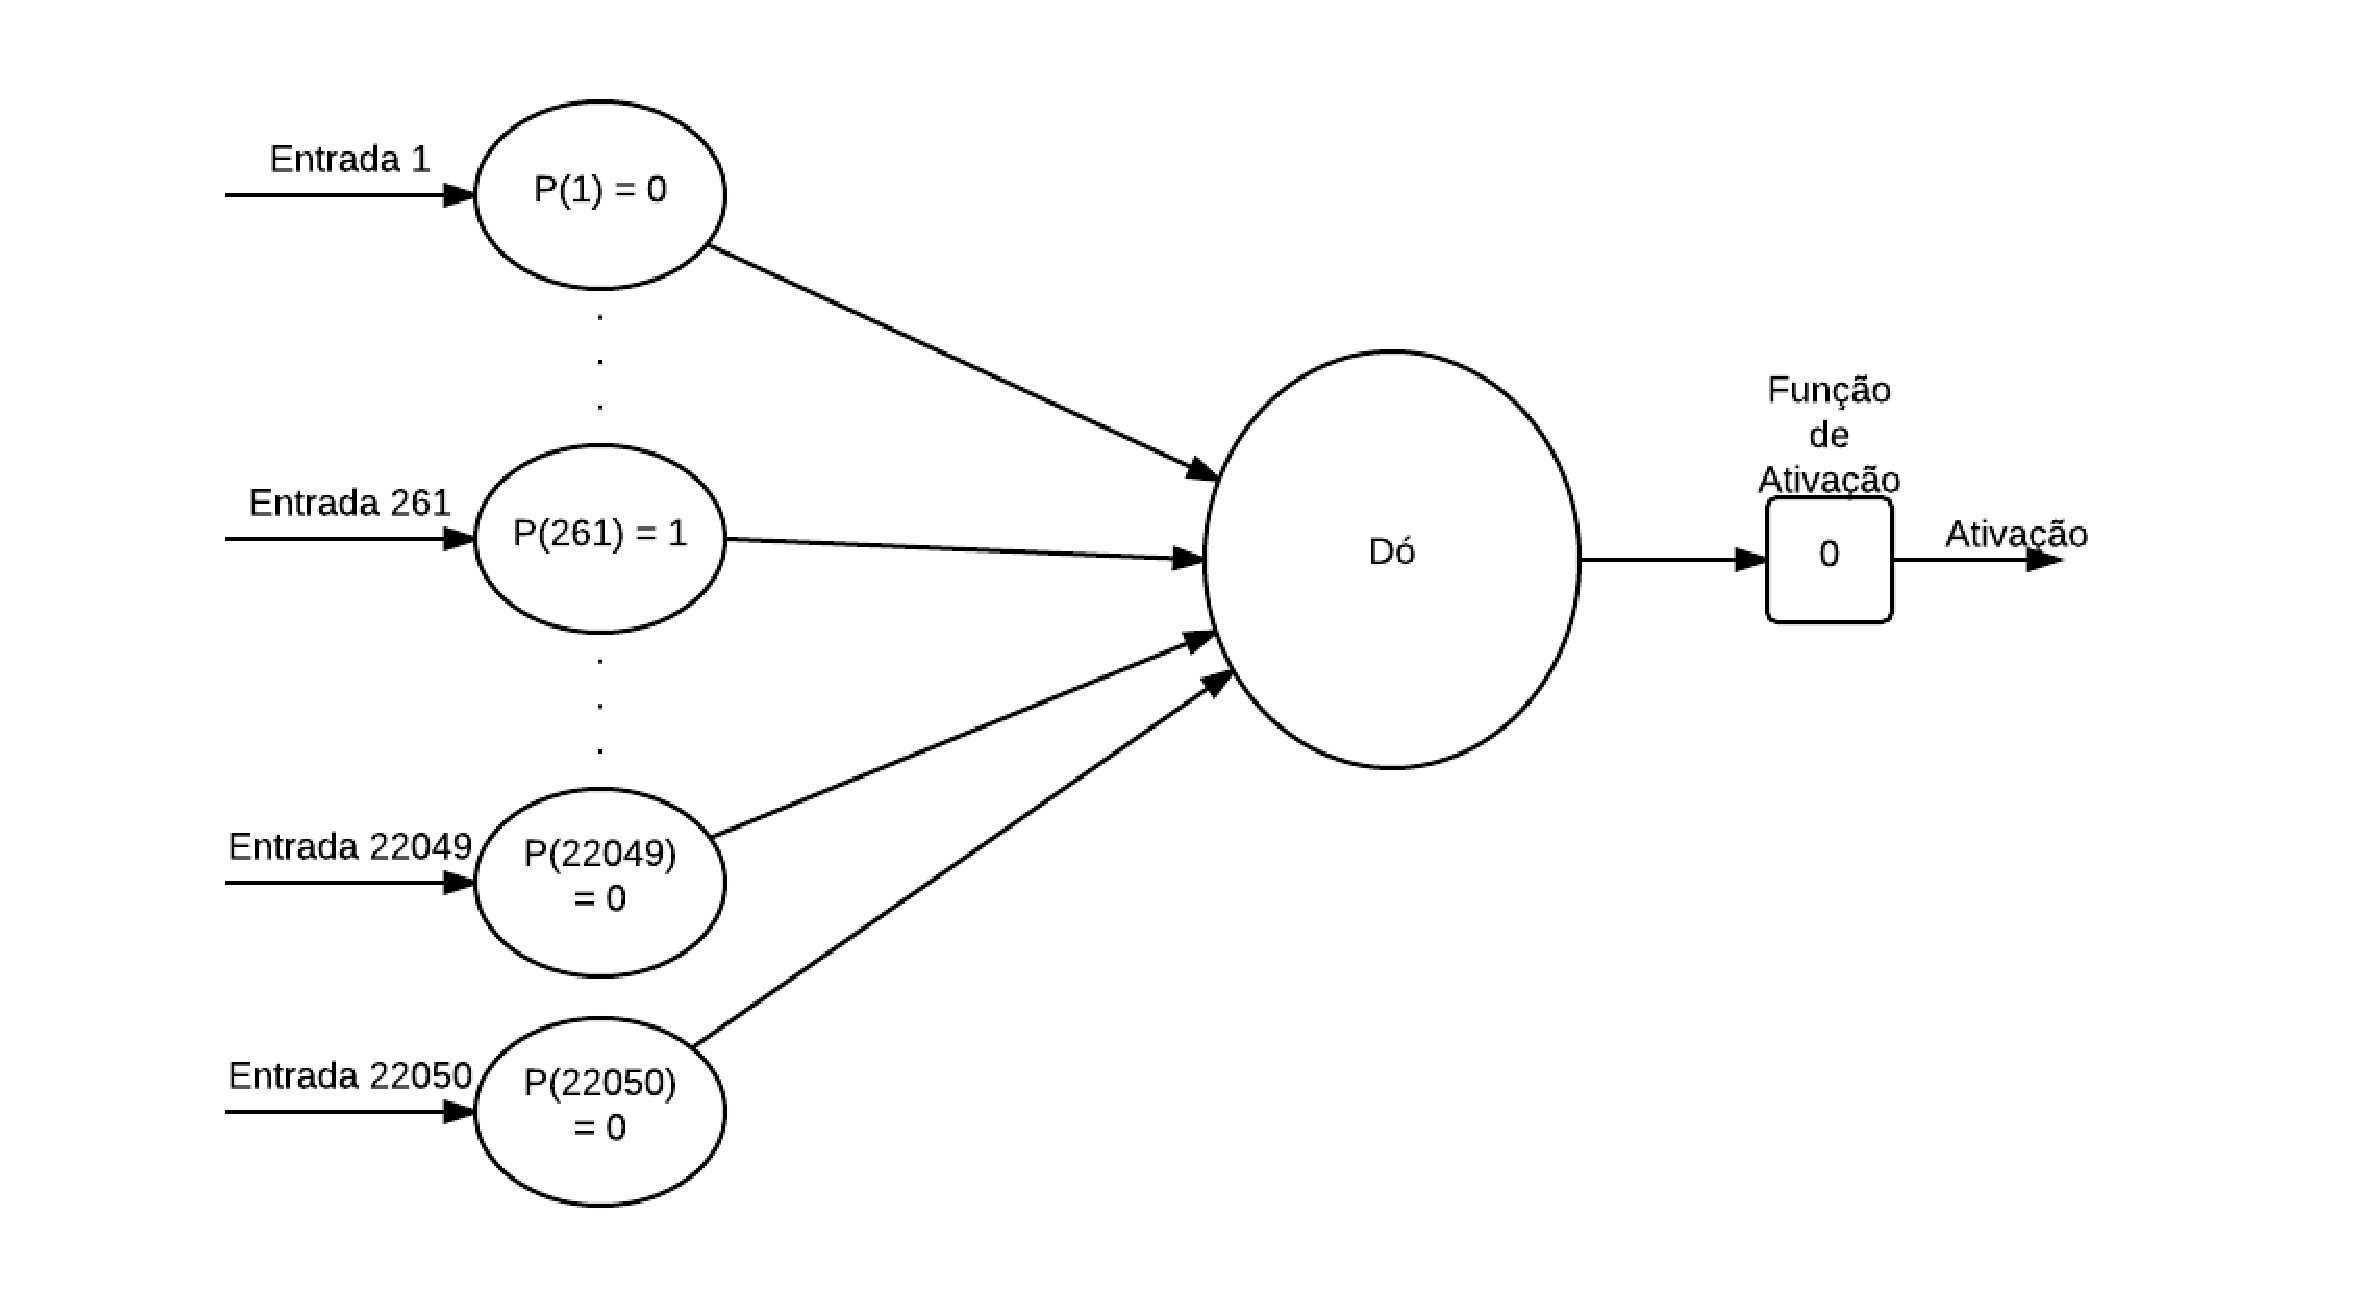
\includegraphics[keepaspectratio=true,scale=0.41]{figuras/neuron_notes}
	\caption{Esquema de Neurônio para Notas}
\end{figure}

Como é mostrado na figura, os neurônios para notas musicais possuem 22050 entradas respectivas a cada frequência. Para cada nota musical há certos pesos diferentes para certas frequências. Os pesos foram obtidos com aprendizagem não-supervisionada, ou seja, não houve nenhum algorítmo de treinamento para a rede. Os pesos foram obtidos por resultados empíricos e são referenciados na seção A.9 dos Apêndices. Os mesmos são gerados no processo de carregar notas.

Para a função de transferência, foi usada a equação de correlação tal qual $x$ é o neurônio constituinte de pesos e $y$ o espectro de frequência do sinal \cite{correlacao}:

\begin{figure}[h]
	\centering
		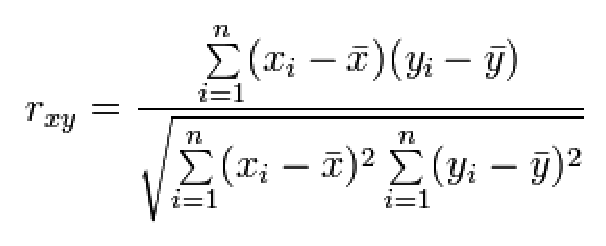
\includegraphics[keepaspectratio=true,scale=0.7]{figuras/correlation-formula}
	\caption{Equação de Correlação}
\end{figure}

Quanto a função de ativação, ela se manteve $f(x)$ $=$ $x$ por motivos de simplificação da aplicação
. Portanto ela é zero, nula ou inexistente.

Para a implementação dessa rede de 12 neurônios segue o código:
\begin{lstlisting}
function S1 = correlate_with_notes(rfeq)
	exec correlation.sci;
	i = 1;
	while (i <= 12)
	    correlacao = coeffcorr(rfeq,notas(i,:));
	    S1(i) = correlacao;
	    i = i + 1;
	end
endfunction
\end{lstlisting}

A função de correleção é nativa do Scilab mas para propósitos didáticos ela está referenciada nos apêndices seção A.6. Nessa estrutura de laço foi calculado cada pontecial de ativação de cada neurônio em relação ao espectro de frequência e guardados na variável \textbf{S1}. Tal vetor pode ser chamado de notas sugeridas.

\section{Correlação com Acordes Musicais}
\label{sec:correlacaoacordes}

Na função de correlacionar as notas musicais sugeridas com acordes há a presença de uma outra estrutura de rede neural. Para essa rede foram criados 48 neurônios, 1 para cada possibilidade de acorde em tríade. Um exemplo de esquema de um neurônio é para o acorde $CM$.

Os neurônios para acordes musicais possuem 12 entradas respectivas a cada nota musical. Para cada acorde musical há certos pesos diferentes para certas notas. Os pesos foram obtidos com aprendizagem não-supervisionada, ou seja, não houve nenhum algorítmo de treinamento para a rede. Os pesos foram obtidos por resultados empíricos e são referenciados na seção A.10 dos Apêndices. Os mesmos são gerados no processo de carregar acordes. Quanto a função de ativação, ela se manteve $f(x)$ $=$ $x$ por motivos de simplificação da aplicação. Portanto ela é zero, nula ou inexistente.

Para a função de transferência, foi usada a mesma equação de correlação para notas musicais. Segue figura ilustrativa do neurônio para o exemplo do acorde de $CM$:

\begin{figure}[t]
	\centering
		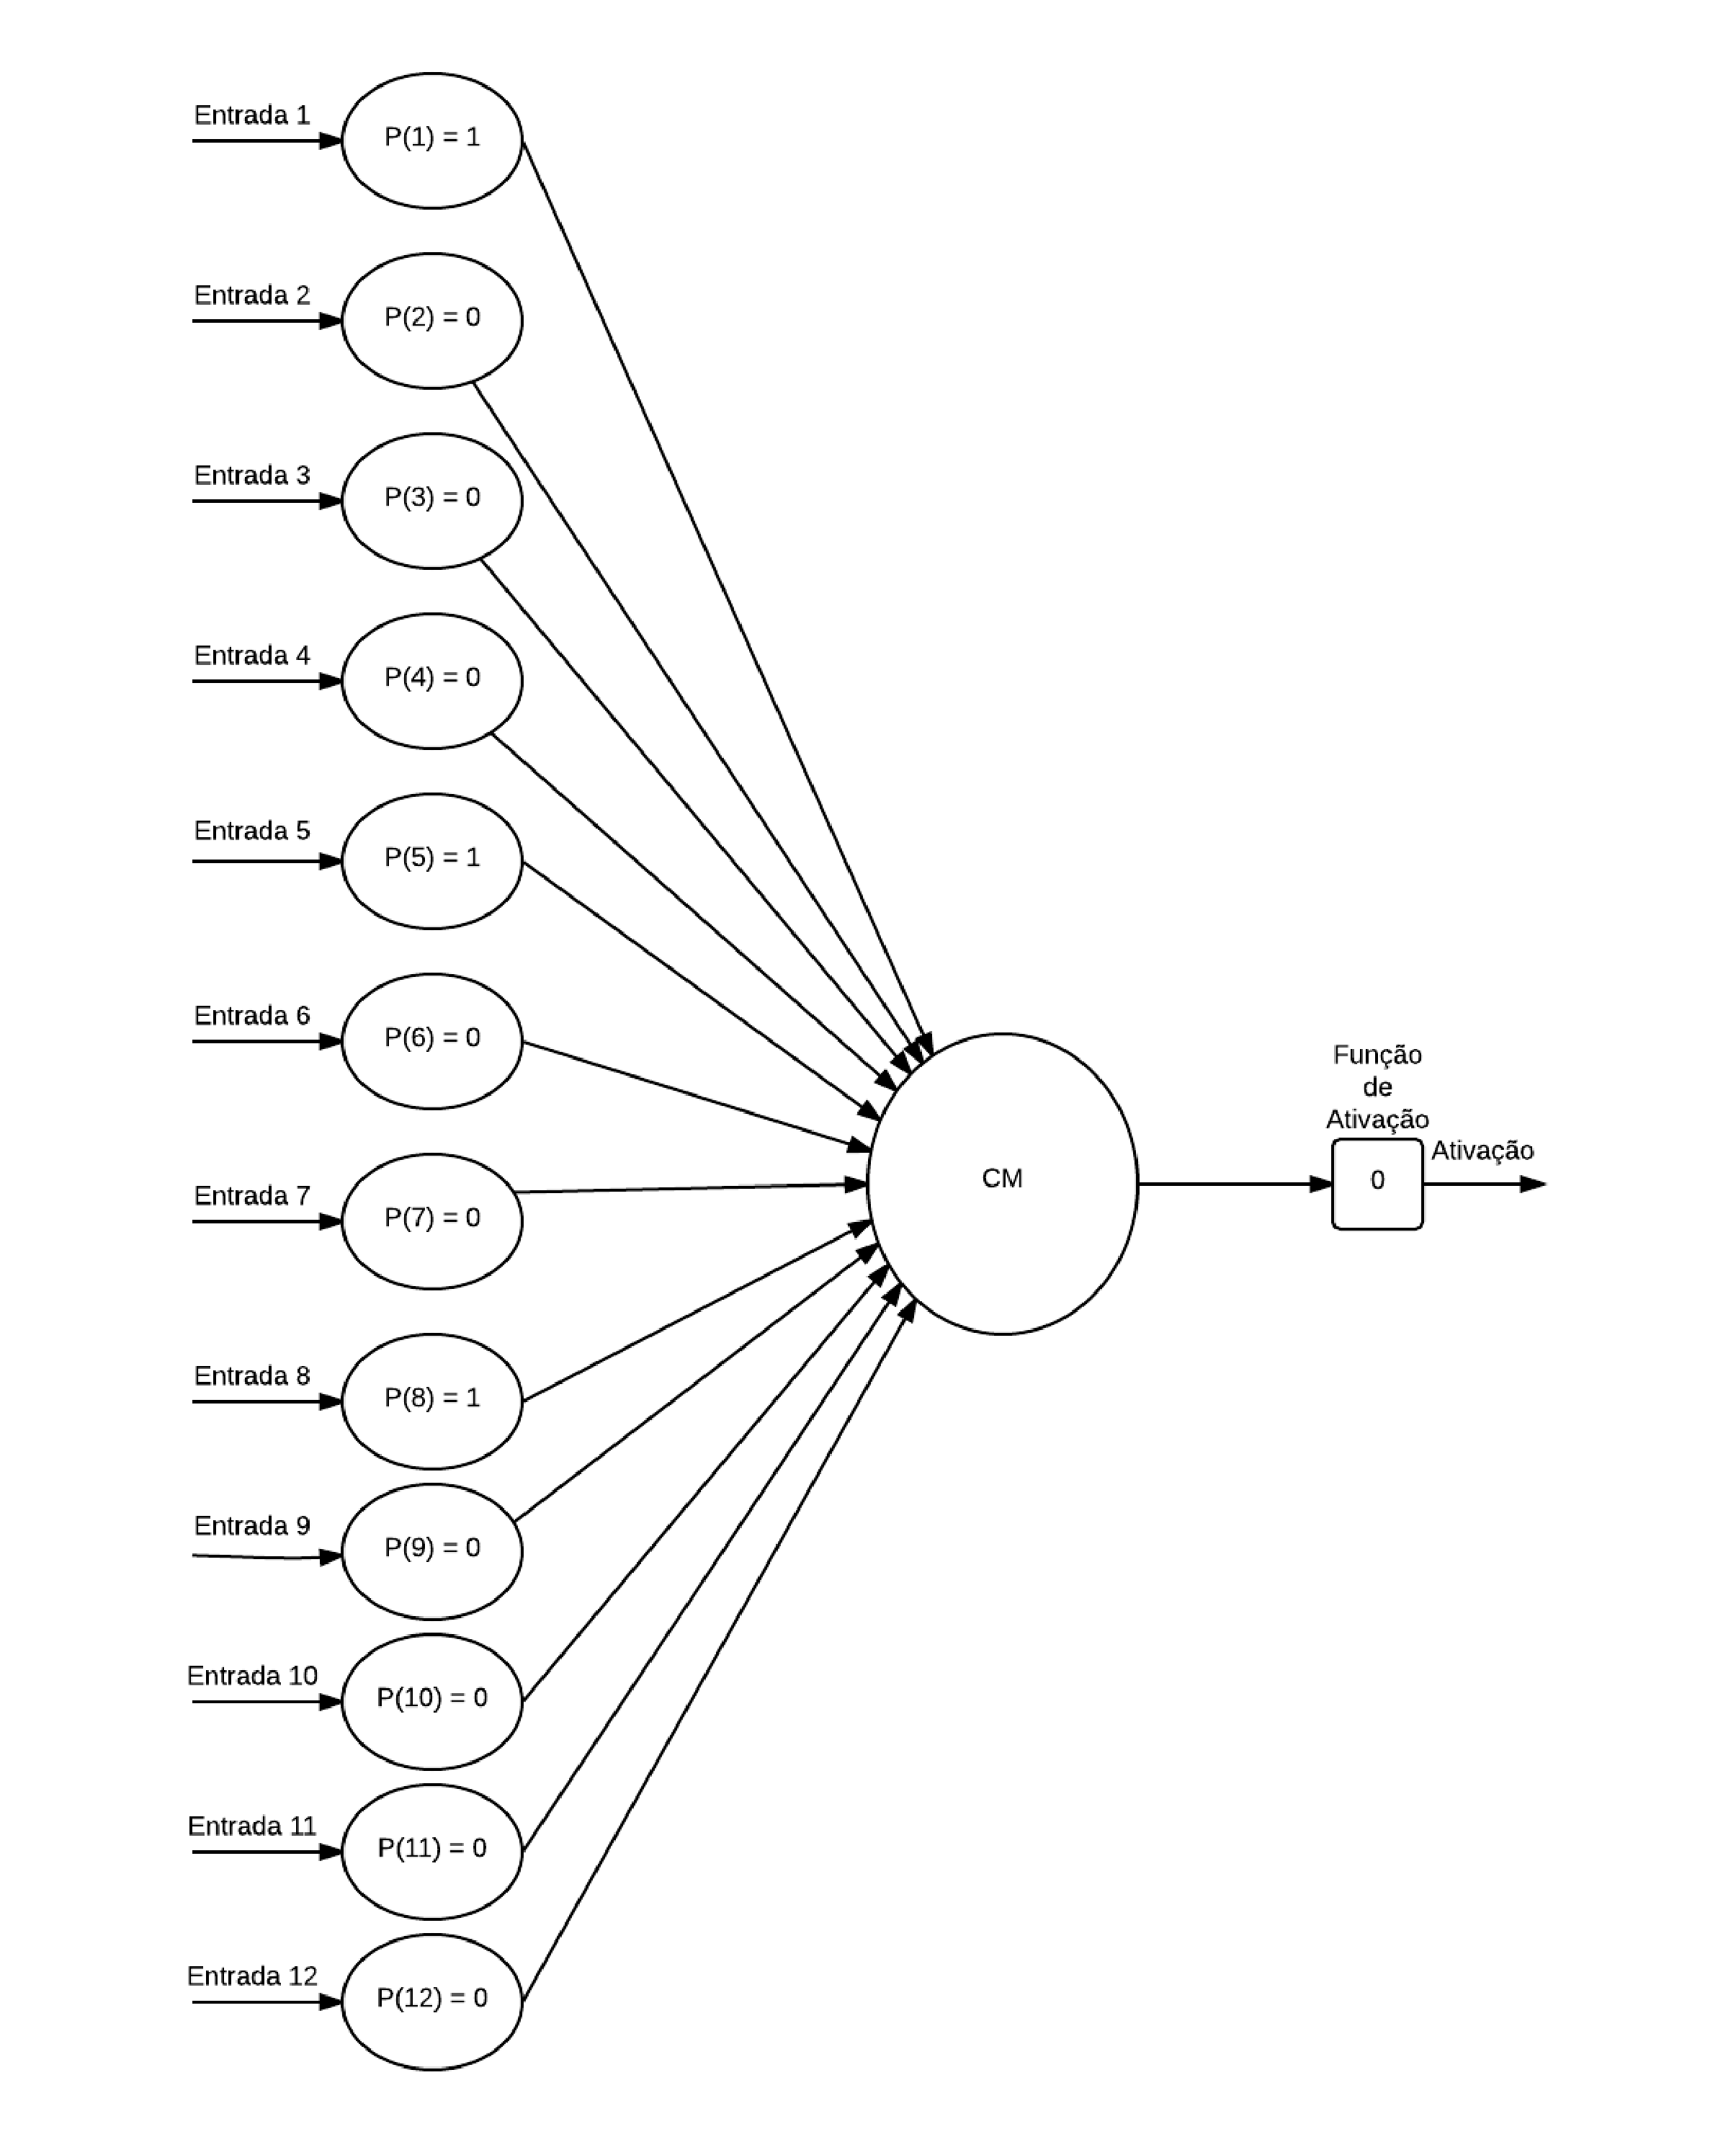
\includegraphics[keepaspectratio=true,scale=0.25]{figuras/neuron_chord}
	\caption{Esquema de Neurônio para Acordes}
\end{figure}


\newpage
Segue código para a rede neural de sugestão de acordes. Assim como a rede neural de notas, a cada iteração há o cálculo da correlação das notas sugeridas com as notas presentes nos acordes já registrados. Os procedimentos podem ser verificados abaixo:

\begin{lstlisting}
function S2 = correlate_with_chords(S1)
	exec correlation.sci;
	i = 1;
	while (i <= 48)
	     correlacao = coeffcorr(S1,BD(:,i)');
	     S2(i) = sqrt(correlacao^2);
	    i = i + 1;
	end
endfunction
\end{lstlisting}

\section{Extração do Acorde}
\label{sec:extracaoacorde}

Para a extração do acorde surgiu a necessidade de implantação da ultima camada da rede. Essa camada é chamada de classificador com máximo, ou seja, ela seleciona o valor máximo entre os impulsos do neurônios. A implementação do classificador de máximos está referenciado na seção A.8 do apêndice.

A nível de arquitetura final da rede neural, segue a ilustração:

\begin{figure}[h]
	\centering
		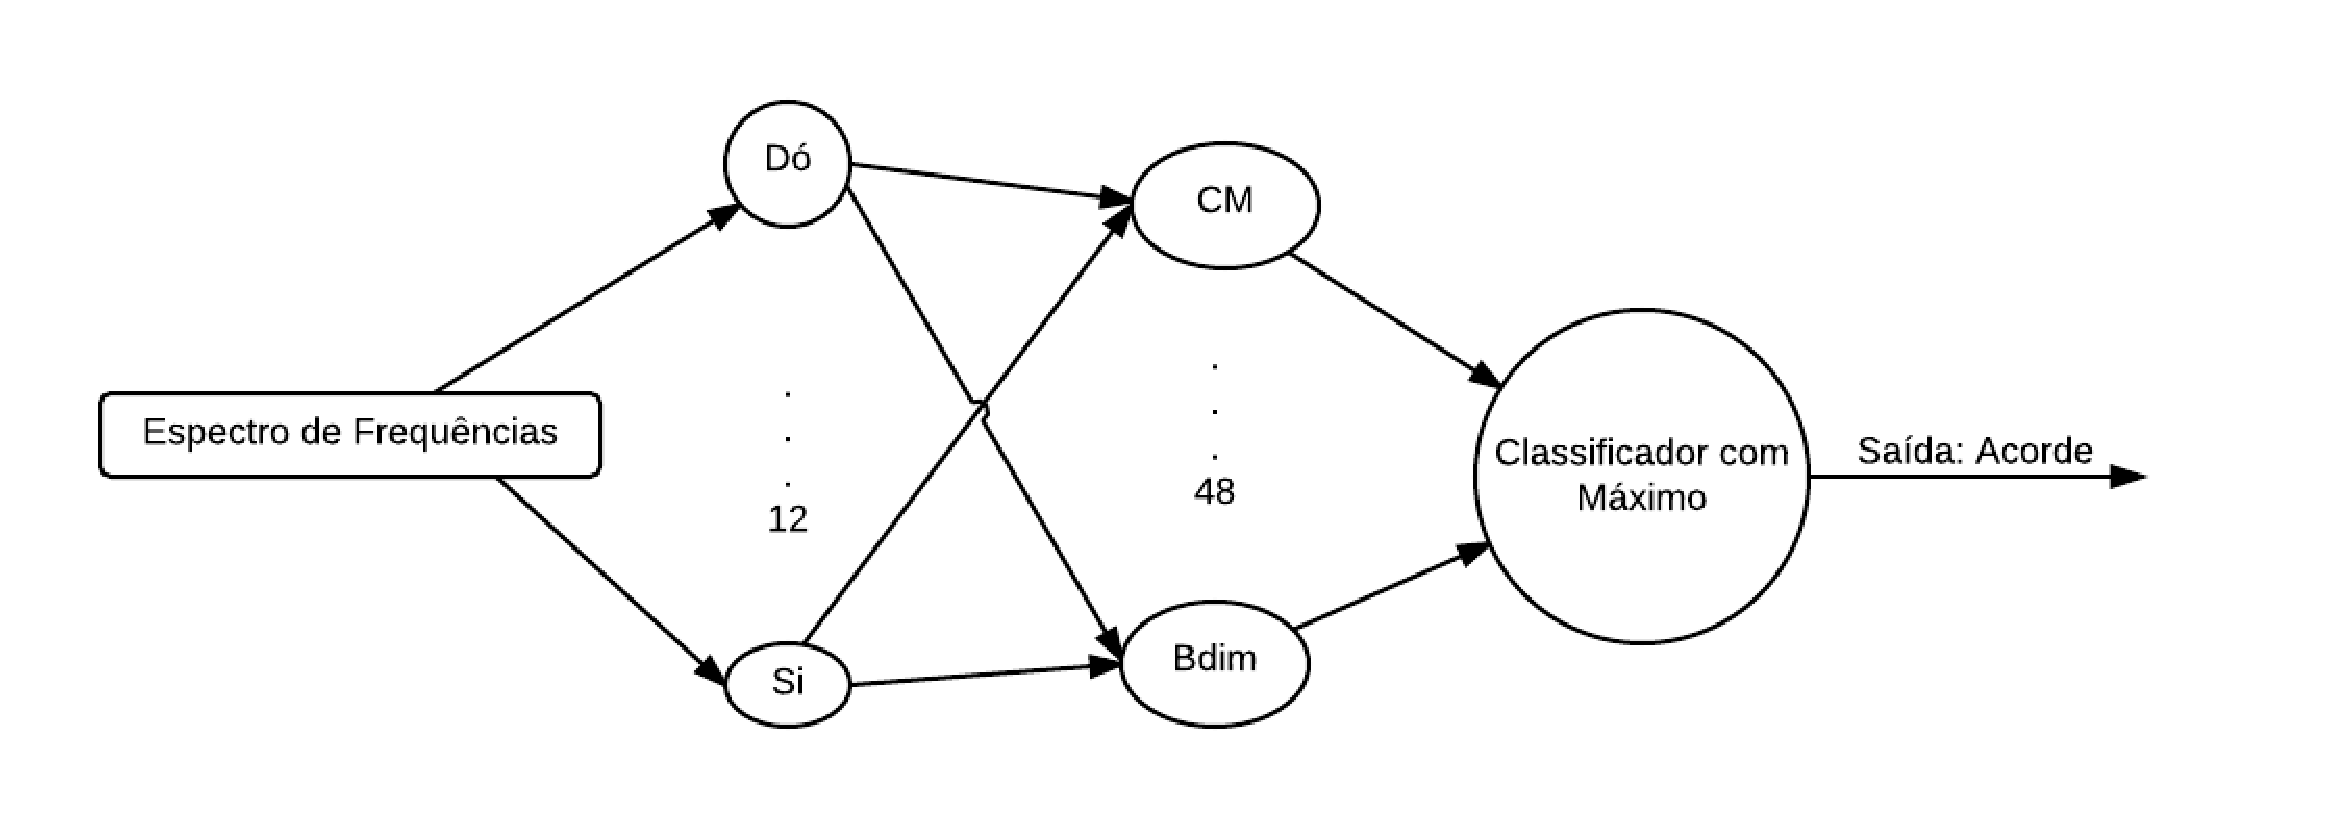
\includegraphics[keepaspectratio=true,scale=0.45]{figuras/rede_total}
	\caption{Esquema da Arquitetura Final da Rede}
\end{figure}

Em tese ela foi embasada na rede neural PNN (Probabilistic Neural Network), porém existem algumas diferenças que foram fundamentais a serem implementadas por conta do contexto. A primeira delas é que a função de transferência de todos os neurônios implementados é uma equação de correleção, pois essa função de transferência se mostrou mais sensível que o a distância euclidiana proposta no modelo padrão, visto que a correlação se embaseia na multiplicação de valores de cada vetor a ser comparado e a distância euclidiana se embaseia numa subtração (para valores pequenos a diferença é muito pequena, ao contrário da multiplicação). Ou seja, a diferença é que as 2 primeiras camadas são padrões em vez da segunda camada ser de soma dos impulsos dos neurônio da camada anterior.
